На кристалл монохроматор (M) падает расходящийся набор рентгеновских лучей, каждый из которых характеризуется отстройкой
$\vartheta$ от точного Брегговского направления (рисунок \ref{ris:triple_crystal_schem}). Отраженный луч с интенсивностью
$I_0 P_M(\vartheta)$ далее падает на образец и дальше $I_0 P_M(\vartheta)P_S(\vartheta)$  на анализатор $I_0 P_M(\vartheta)P_S(\vartheta)P_A(\vartheta)$,
сохраняя величину отстройки.

Необходимо также ввести угловые отстройки от точного брегговского положения
для образца (S) $\theta$ и анализатора (A) $\varepsilon$  (углы отсчитываются в сторону увеличения угла падающего луча).
В результате поворота образца на угол  $\theta$ излучение отраженное от монохроматора, падает на образец
под углом $\theta_B+\theta+\vartheta$. Если кристалл повернуть на угол $\theta$, отраженный повернется на удвоенный угол
$2\theta$, в итоге излучение падает на анализатор (А) под углом $\theta_B+2\theta-\varepsilon+\vartheta$ \cite{trd_Bushuev_1997}.
\begin{figure}[H]
  \centering
  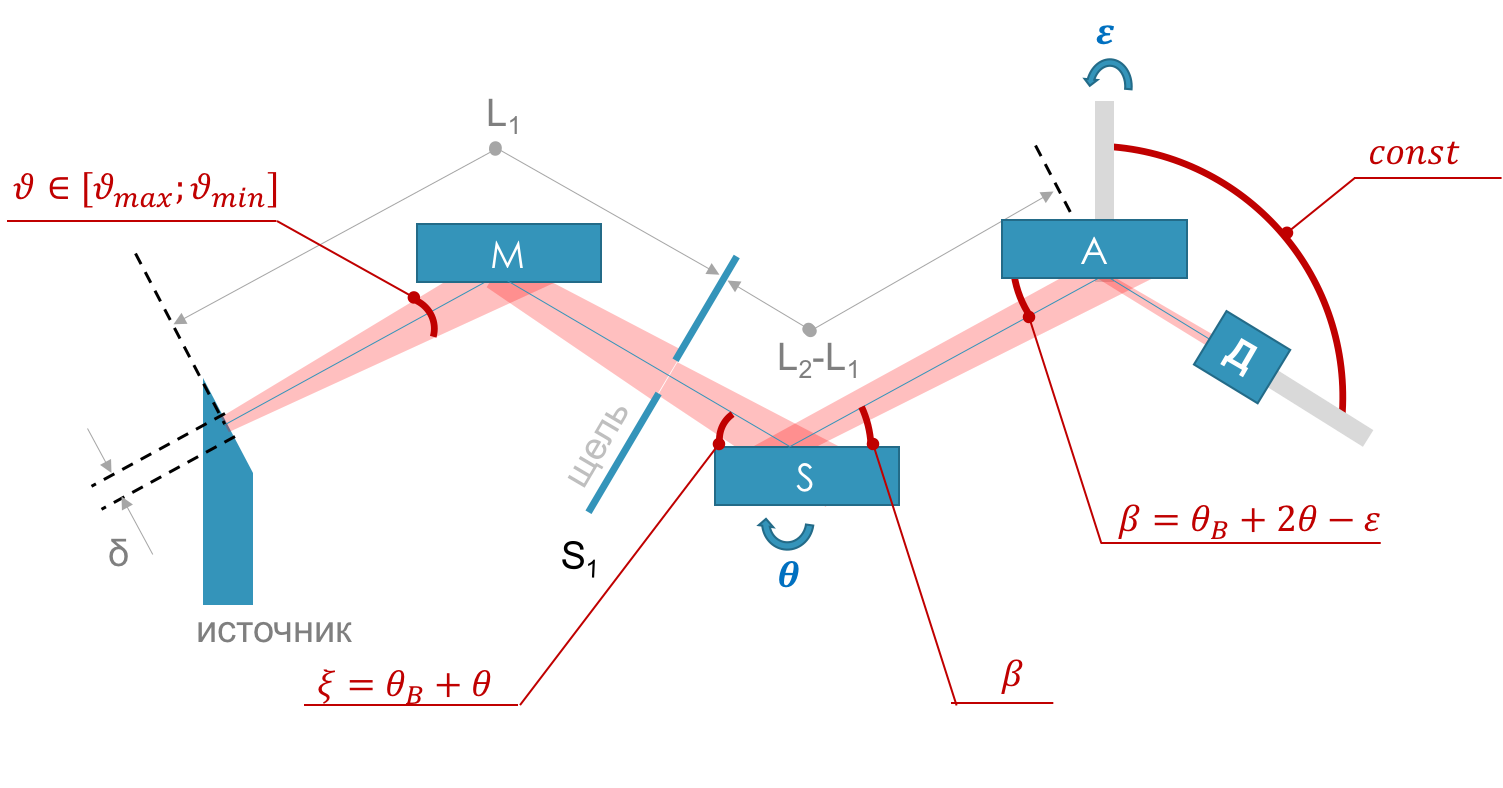
\includegraphics[width=0.8\textwidth]{images/triple_crystal_schem.png}
  \caption{Схема трехкристального эксперимента, $\theta$ - отстройка образца от точного угла Брегга,
  $\varepsilon$ - угол отстройки анализатора относительно положения оптической оси}
  \label{ris:triple_crystal_schem}
\end{figure}

Учитывая что рентгеновская трубка имеет полихроматический спектр, лучи падающие под разными углами могут отражаться
с одинаковым коэффициентом отражения за счет разной энергии $\frac{\lambda - \lambda_1}{\lambda_1}\tan(\theta_B)$,
спектрально угловое распределение, исходя из вышесказанного, задается выражением:

\begin{eqnarray} \label{eq:triplr_spectra_angle_map}
  P_{triple}(\vartheta,\lambda,\theta,\varepsilon) =I_0\cdot
    P_M \left(\vartheta - \frac{\lambda - \lambda_1}{\lambda_1}\tan(\theta_B) \right) \cdot \nonumber \\
   P_S \left(\theta + \vartheta - \frac{\lambda - \lambda_1}{\lambda_1}\tan(\theta_B)\right)  \cdot  \nonumber \\
   P_A \left(2\theta - \varepsilon + \vartheta - \frac{\lambda - \lambda_1}{\lambda_1}\tan(\theta_B)\right) \Bigg]
 \end{eqnarray}

  \begin{figure}[H]
    \centering
    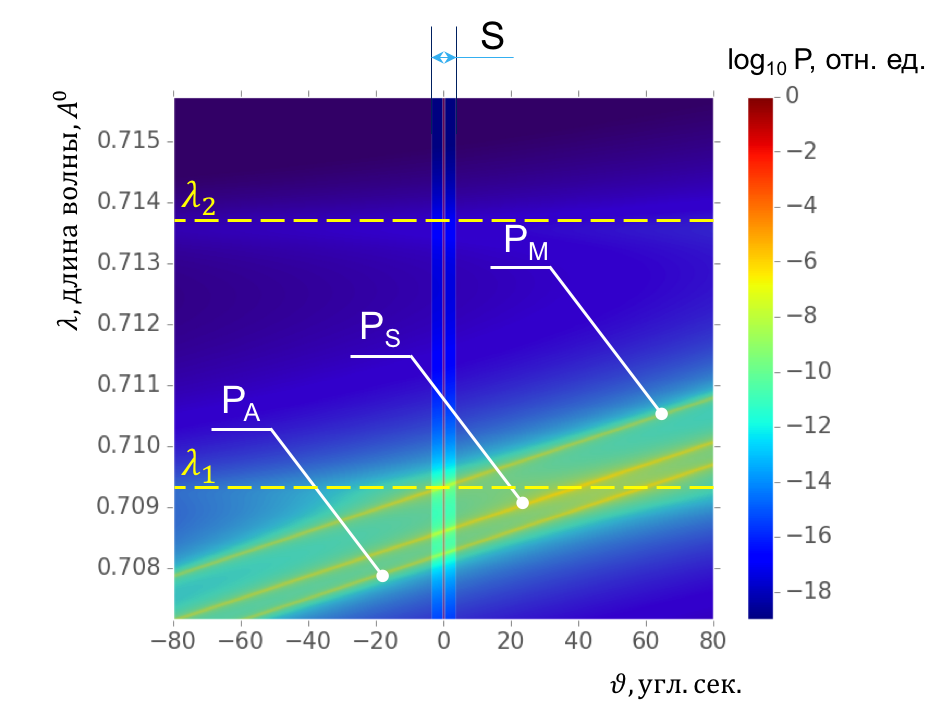
\includegraphics[width=0.6\textwidth]{images/triple_map.png}
    \caption{Спектрально-угловое распределение в случае наличия трех кристаллов в схеме для
    лабораторного источника с молибденовым анодом.
    Прямая образца отстроена на $\theta = - 50''$, анализатора на $\varepsilon = 20''$ относительно
    зеркально отраженного луча после кристалла-образца. Так же на схеме изображено щелевое устройство размером около 7 $''$}
    \label{ris:triple_map}
  \end{figure}

Анализ движения прямых отражения на спектрально-угловом распределении (рисунок \ref{ris:triple_map}) от угла отстройки образца $\theta$ и
анализатора $\varepsilon$ показывает, что суммарная интенсивность зафиксированная детектором внутри щелевого устройства
$S$ имеет вид пикообразной кривой состоящей из трех максимумов (рисунок \ref{ris:triple_map_piks}).

\begin{figure}[H]
  \centering
  \subfloat[главный пик]{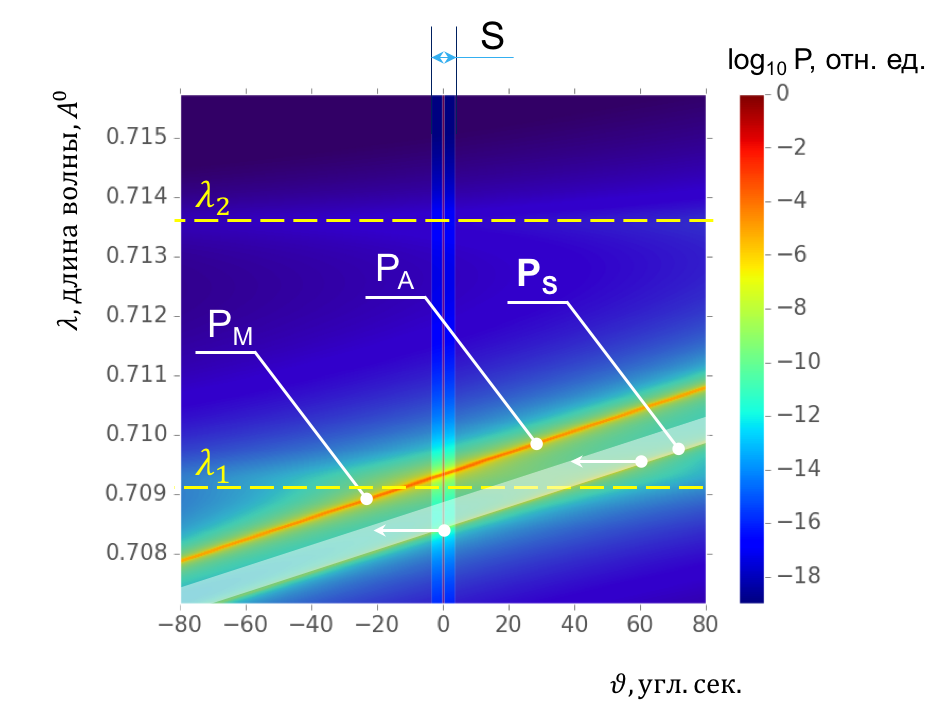
\includegraphics[width=0.325\textwidth]{images/triple_map_g.png}\label{ris:triple_map_piks_g}}
  \hfill
  \subfloat[псевдо пик монохроматора]{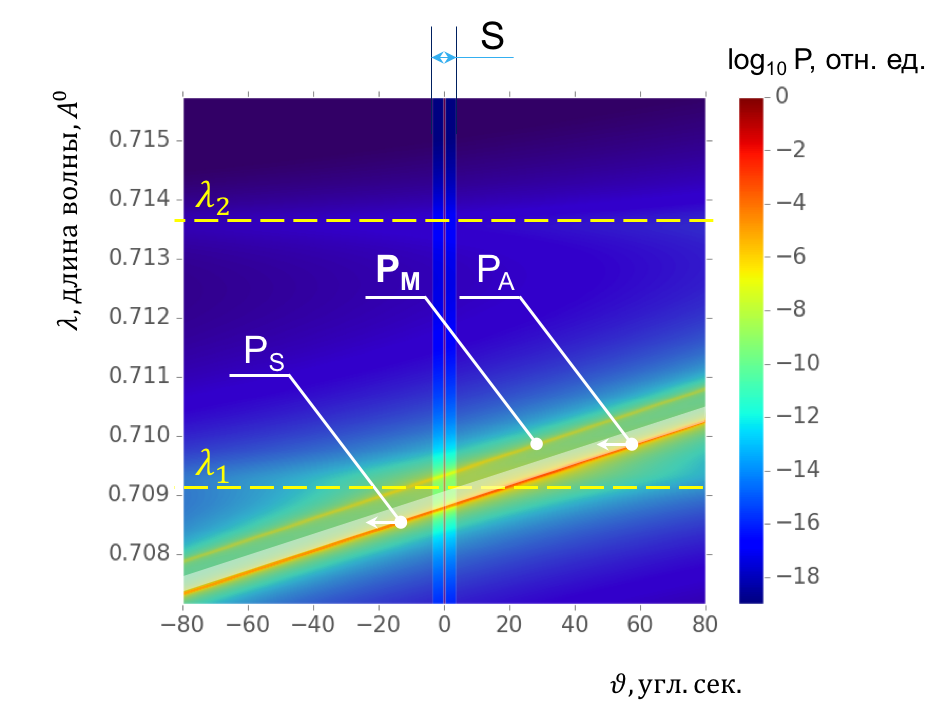
\includegraphics[width=0.325\textwidth]{images/triple_map_m.png} \label{ris:triple_map_piks_m}}
  \hfill
  \subfloat[псевдо пик анализатора]{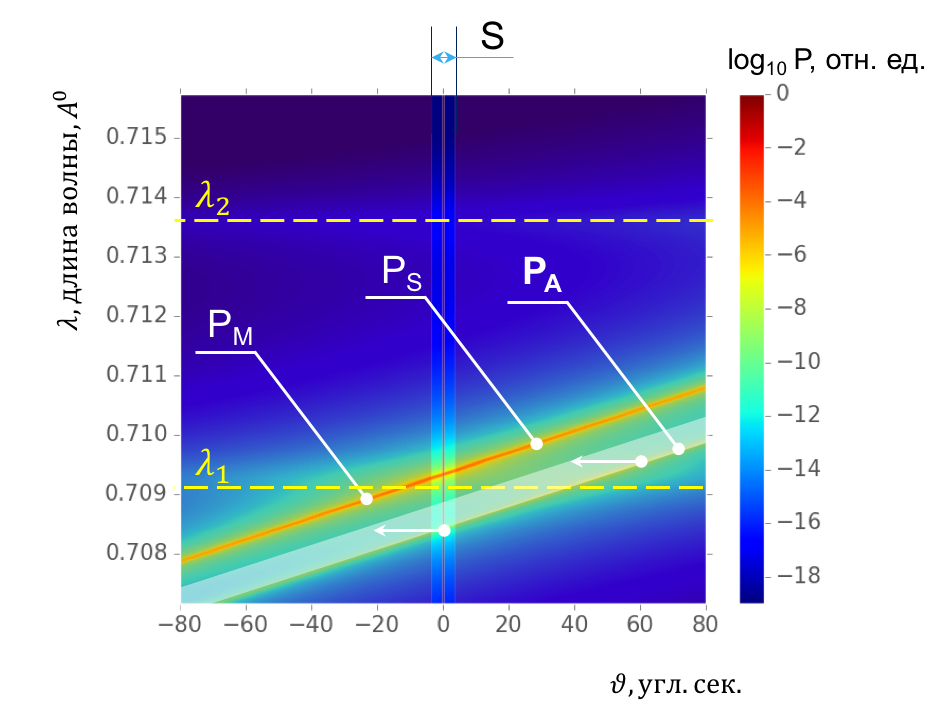
\includegraphics[width=0.325\textwidth]{images/triple_map_a.png} \label{ris:triple_map_piks_a}}
  \caption{Формирование карты рассеяния в прямом пространстве}
  \label{ris:triple_map_piks}
\end{figure}


\subsubsection*{Главный пик}
Главный пик (ГП) формируется в случае отстройки кристалла-образца от точного угла Брегга,
максимум при $|\theta|>>0''$ имеет место при повороте анализатора на $\varepsilon = 2\theta$,
тогда выражение (\ref{eq:triplr_spectra_angle_map}) примет частный вид

\begin{eqnarray} \label{eq:triplr_spectra_angle_map_GP}
  P_{\text{ГП}}(\vartheta,\lambda,\theta,\varepsilon) =I_0\cdot
    P_M \left(\vartheta - \frac{\lambda - \lambda_1}{\lambda_1}\tan(\theta_B) \right) \cdot \nonumber \\
   P_S \left(\theta + \vartheta - \frac{\lambda - \lambda_1}{\lambda_1}\tan(\theta_B)\right)  \cdot  \nonumber \\
   P_A \left(0+\vartheta - \frac{\lambda - \lambda_1}{\lambda_1}\tan(\theta_B)\right) \Bigg]
 \end{eqnarray}
как видно на рис. \ref{ris:triple_map_piks_g}, прямая анализатора и образца перекрывают друг друга и пик формируется
движением прямой образца. Такой режим сканирования в экспериментальной практике называется $\theta-2\theta$ сканированием,
угол поворота кристалла образца соответствует удвоенному повороту анализатора. В этом случае мы движемся
вдоль пика чисто когерентного рассеяния, т.е. направляя на образец луч с конкретными значением отстройки $\vartheta$ и энергией соответствующей
 $\lambda$, а дальше анализируем отраженный луч, с той же энергией и угловой составляющей. Для примера, это
 будет показано дальше, образец с измененным межплоскостным расстоянием будет смещать максимум отражения именно вдоль направления
 главного (когерентного) пика.

\subsubsection*{Пседво пик монохроматора}
Псевдо пик монохроматора (ППМ) (рисунок \ref{ris:triple_map_piks_m}) формируется в случае когда прямые образца и анализатора
двигаются вместе, перекрываясь между собой. Угол отстройки образца и анализатора совпадает $\theta = \varepsilon$.

\begin{eqnarray} \label{eq:triplr_spectra_angle_map_PPM}
  P_{\text{ППМ}}(\vartheta,\lambda,\theta,\varepsilon = \theta) =I_0\cdot
    P_M \left(\vartheta - \frac{\lambda - \lambda_1}{\lambda_1}\tan(\theta_B) \right) \cdot \nonumber \\
   P_S \left(\theta + \vartheta - \frac{\lambda - \lambda_1}{\lambda_1}\tan(\theta_B)\right)  \cdot  \nonumber \\
   P_A \left(\theta  + \vartheta - \frac{\lambda - \lambda_1}{\lambda_1}\tan(\theta_B)\right) \Bigg]
 \end{eqnarray}

 \subsubsection*{Пседво пик анализатора}
 Псевдо пик анализатора (ППА) формируется в случае когда монохроматор и образец
 находятся в точном брегговском положении, перекрываясь между собой. Движение вдоль ППА осуществляется
 движением анализатора  на карте спектрально углового распределения (рисунок \ref{ris:triple_map_piks_a}).
   Угол отстройки образца и анализатора совпадает $\theta = 0$.

 \begin{eqnarray} \label{eq:triplr_spectra_angle_map_PPM}
   P_{\text{ППА}}(\vartheta,\lambda,\theta=0,\varepsilon) =I_0\cdot
     P_M \left(\vartheta - \frac{\lambda - \lambda_1}{\lambda_1}\tan(\theta_B) \right) \cdot \nonumber \\
    P_S \left(0 + \vartheta - \frac{\lambda - \lambda_1}{\lambda_1}\tan(\theta_B)\right)  \cdot  \nonumber \\
    P_A \left(0-\varepsilon  + \vartheta - \frac{\lambda - \lambda_1}{\lambda_1}\tan(\theta_B)\right) \Bigg]
  \end{eqnarray}


\subsubsection*{Интенсивность на детекторе}

Учтем теперь, что детектирующее устройство суммирует всю интенсивность в пределах своей аппертуры и по всем длина волн,
таким образом выражения для распределения интенсивности в методе трехкристальной рентгеновской дифракции имеет следующий
общий вид:

\begin{eqnarray} \label{eq:doudle_spectra_angle}
  P_{triple}(\theta,\varepsilon) = \sum_{\lambda = -\infty}^{\infty}g_{\lambda}(\lambda)\cdot
  \sum_{\vartheta = \vartheta_{s1}}^{\vartheta_{s2}} \Bigg[ g_{\vartheta}(\vartheta) g_{S}(\vartheta) \cdot \nonumber \\
    P_M \left(\vartheta - \frac{\lambda - \lambda_1}{\lambda_1}\tan(\theta_B) \right) \cdot \nonumber \\
   P_S \left(\theta + \vartheta - \frac{\lambda - \lambda_1}{\lambda_1}\tan(\theta_B)\right)  \cdot  \nonumber \\
   P_A \left(2\theta - \varepsilon + \vartheta - \frac{\lambda - \lambda_1}{\lambda_1}\tan(\theta_B)\right) \Bigg]
 \end{eqnarray}
где пределы суммирования определяются щелевым коллиматором $\vartheta_{s2} = - \vartheta_{s1} = \frac{\delta+S_1}{2L_1}$.
 \begin{figure}[H]
   \centering
   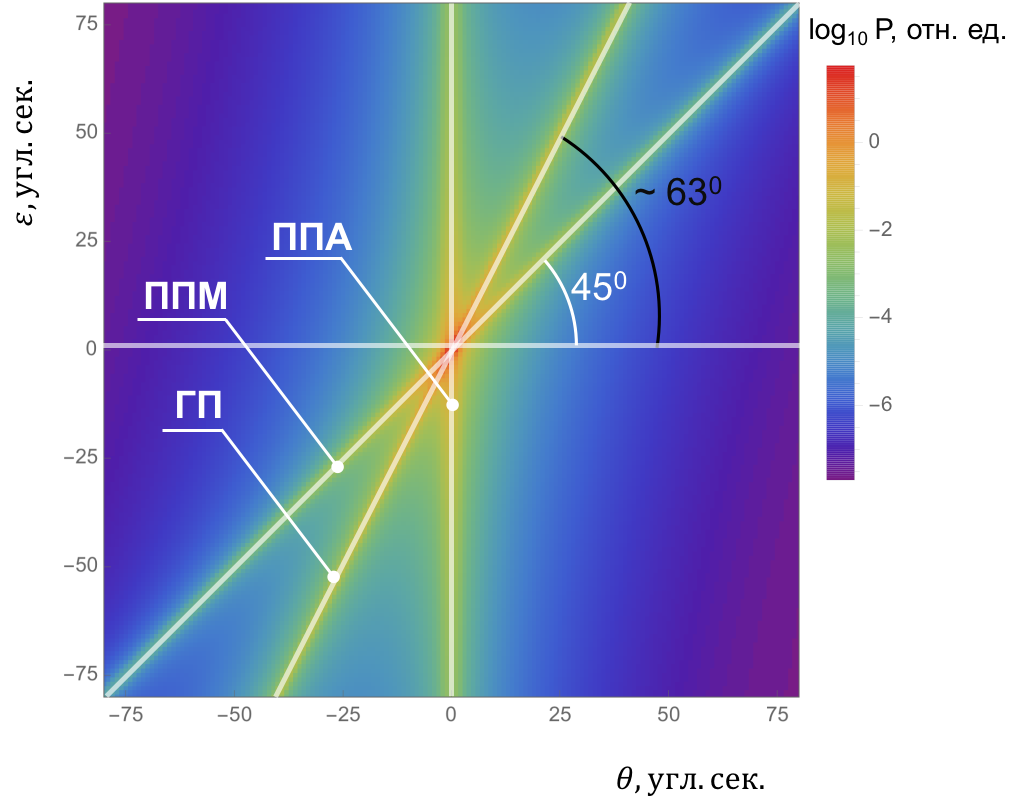
\includegraphics[width=0.6\textwidth]{images/triple_map_direct_space.png}
   \caption{Трехкристальная карта распределения в пространстве углов отстройки $\theta$ - образца и $\varepsilon$
   -  анализатора.}
   \label{ris:triple_map_direct_space}
 \end{figure}

Анализ показывает, что ГП находится под углом $60^o$, т.к. сканирование осуществляется вдоль $\varepsilon = 2 \theta$,
а $ \arctan \left(\frac{\varepsilon}{\theta} \right) = 63.4^o$. ППМ образует угол $45^o$, т.к. $\varepsilon = \theta$.
